\documentclass[conference]{IEEEtran}

\usepackage{cite}
\usepackage{amsmath,amssymb,amsfonts}
\usepackage{algorithmic}
\usepackage{graphicx}
\usepackage{textcomp}
\usepackage{xcolor}

\usepackage{custom}

% \makeglossaries
\newacronym{ast}{AST}{Application Security Testing}

\newacronym{dast}{DAST}{Dynamic Application Security Testing}

\newacronym{sast}{SAST}{Static Application Security Testing}

\newacronym{iast}{IAST}{Interactive Application Security Testing}

\newacronym{sca}{SCA}{Software Composition Analysis}

\newacronym{iac}{IaC}{Infrastructure as Code}

\newacronym{sdlc}{SDLC}{Software Development Life Cycle}

\newacronym{owasp}{OWASP}{Open Worldwide Application Security Project}

\newacronym{zap}{ZAP}{Zed Attack Proxy}

\newacronym{soc}{SoC}{System-on-Chip}

\newacronym{www}{WWW}{World Wide Web}

\newacronym{wasm}{WASM}{WebAssembly}

\newacronym{cli}{CLI}{Command Line Interface}

\newacronym{zesti}{ZESTI}{Zero-Effort Symbolic Test Improvement}

\newacronym{spf}{SPF}{Symbolic PathFinder}

\newacronym{jpf}{JPF}{Java PathFinder}

\newacronym{cdse}{CDSE}{Con\-flict-Driven Symbolic Execution}


\begin{document}

\title{Comparative study of symbolic execution tools applied to vulnerability detection}

\author{\IEEEauthorblockN{André Cardoso}
\IEEEauthorblockA{\textit{School of Technology} \\
\textit{Polytechnic Institute of Cávado and Ave}\\
Barcelos, Portugal \\
a18848@alunos.ipca.pt}
\and
\IEEEauthorblockN{Nuno Lopes}
\IEEEauthorblockA{\textit{2AI - School of Technology, IPCA} \\
Barcelos, Portugal \\
\textit{LASI - Associate Laboratory of Intelligent Systems}\\
Guimarães, Portugal \\
0000-0001-8897-5061}
% \and
% \IEEEauthorblockN{3\textsuperscript{rd} Given Name Surname}
% \IEEEauthorblockA{\textit{dept. name of organization (of Aff.)} \\
% \textit{name of organization (of Aff.)}\\
% City, Country \\
% email address or ORCID}
% \and
% \IEEEauthorblockN{4\textsuperscript{th} Given Name Surname}
% \IEEEauthorblockA{\textit{dept. name of organization (of Aff.)} \\
% \textit{name of organization (of Aff.)}\\
% City, Country \\
% email address or ORCID}
% \and
% \IEEEauthorblockN{5\textsuperscript{th} Given Name Surname}
% \IEEEauthorblockA{\textit{dept. name of organization (of Aff.)} \\
% \textit{name of organization (of Aff.)}\\
% City, Country \\
% email address or ORCID}
% \and
% \IEEEauthorblockN{6\textsuperscript{th} Given Name Surname}
% \IEEEauthorblockA{\textit{dept. name of organization (of Aff.)} \\
% \textit{name of organization (of Aff.)}\\
% City, Country \\
% email address or ORCID}
}

\maketitle

\begin{abstract}
The security of an application showed to be a critical aspect of software development, and one way to test for vulnerabilities is through symbolic execution.

This paper will present a comparative study of two symbolic execution tools, KLEE and Owi, applied to vulnerability detection in software applications. After experimenting with both tools, and analysing the results, it's noted better performance and more comprehensive results with KLEE.
\end{abstract}

\begin{IEEEkeywords}
Symbolic Execution, Application Security Testing, Static Code Analysis, KLEE, Owi
\end{IEEEkeywords}


\section{INTRODUCTION} \label{chap:intro}
The security of an application showed its first impacts around the beginning of the century with the increasing popularity of the \glsxtrfull{www} and the enablement of user-fuelled websites (like social media). This rapid evolution paired with the common lack of knowledge of the users but also of the developers caused the birth of Denial of Service and Cross-Site Scripting attacks among others \cite{Hoffman2024}.

% In the digital era, it is evident that most individuals interact with devices running software that may be susceptible to exploitation. A fundamental principle in cybersecurity is that all software contains vulnerabilities; therefore, its security posture depends primarily on the difficulty of detection. The risk of attack correlates with the diligence of security teams in remediation efforts and the potential incentives available to attackers.

% \subsection{Motivation and Background}
% Considering this, software organizations must take action in defending their codebases in the most efficient manner when it comes to resources and time. Manual validations are based in human interaction, which is known to be very prone to errors, making it not cost-efficient. Also, as an application evolves in complexity, manual validation is not viable when it comes to the resources required, but also time as this is an operation that requires celerity. This procedure is often described as \glsxtrfull{ast}.

As such, many tools to find vulnerabilities in an automated fashion have been developed and distributed, each with their own set of pros and cons. The tools in question can be categorized as static or dynamic, and each on their own use different technics to accomplish different results. \glsxtrfull{sast} ultimately relies on some variety of pattern matching, data-flow analysis, and symbolic execution \cite{Croft2021},%, while \glsxtrfull{dast} excels at mimicking realistic attacks and threats \cite{DAST_description}.

% \subsection{Objectives}\label{section:objectives}
The objective is a comparison of two symbolic execution tools and see how they compare in terms of performance and their ability to detect vulnerabilities. To achieve this comparison, the tools must run on projects that are preferably coded in the same language, but if these tools do not support the same set of languages, the projects should have similar architecture or business logic/intent (e.g.: online stores, accounting services, ...). These tools will also be compared on how they can be tuned in order to achieve better results.

For a better overview of how the comparison will be performed, here follows a set of questions and metrics used to measure the tools:
\begin{itemize}
    \item Time to test a project
    \item CPU usage while testing a project
    \item Memory usage while testing a project
    \item Analysis of vulnerabilities detection (Youden's Index)
    \item Complexity of the vulnerabilities detected
    \item Ability to find vulnerabilities out-of-the-box
    \item Ability to find vulnerabilities with proper manipulation
    \item Effort of tuning the tool
\end{itemize}

In sum, the expected output is a clear comparison of tools that can assist developers and software companies in keeping code secure proactively and explain what differs between them and why one should pick one over the other(s). These is how we intend to answer the following research questions:

\begin{itemize}
    \item \textbf{Which tool is more effective at finding vulnerabilities?}
    \item \textbf{Which tool is more efficient in terms of performance?}
\end{itemize}

% \subsection{Research Method}\label{section:research_method}

% Design-Science Research is the most suitable research method for this work as it focuses on the creation and evaluation of artifacts that solve identified organizational problems \cite{Hevner2004}. In this case, the organizational problem is the need for efficient and effective tools to identify vulnerabilities in software applications, which is a critical concern for software development organizations aiming to enhance their security posture.

% \cite{Hevner2004} outlines 7 guidelines for conducting Design-Science Research, which will be followed in this study:
% \begin{enumerate}
%     \item \textbf{Design as an Artifact:} The primary artifacts in this research is the research itself - a comparative analysis of symbolic execution tools for vulnerability detection - and the repository with the samples used in the experiments (see \cref{chap:experiences}). 
%     \item \textbf{Problem Relevance:} The research addresses the practical problem of identifying effective symbolic execution tools for vulnerability detection in software applications. This research also guides practitioners in the setup and usage of these tools (see \cref{chap:symbolic_execution_tools}).
%     \item \textbf{Design Evaluation:} The evaluation of the symbolic execution tools will be conducted through empirical testing on selected software projects, measuring performance metrics and vulnerability detection capabilities (see \cref{chap:experiences}).
%     \item \textbf{Research Contributions:} The study aims to contribute to the field of software security by providing insights into the effectiveness and efficiency of different symbolic execution tools and offering guidance for practitioners in selecting appropriate tools (see \cref{chap:experiences}, particularly \cref{section:results}).
%     \item \textbf{Research Rigor:} The research will employ rigorous methodologies for tool selection, testing, and data analysis to ensure the validity and reliability of the findings (see \cref{section:test_environment}).
%     \item \textbf{Design as a Search Process:} The research will involve an iterative process of tool selection, testing, and refinement to identify the most effective and/or efficient symbolic execution tools (\cref{subsection:symbolic_exec_engines,section:engines_availability,chap:experiences}).
%     \item \textbf{Communication of Research:} The findings of the research will be documented and disseminated through academic publications and presentations to reach both the academic community and industry practitioners. This document serves as the primary medium for communicating the research process and findings, and the testing is shared in a public repository (url: \url{https://github.com/18848/masters_thesis}).
% \end{enumerate}

% The comparison of symbolic execution tools can be summed up by the question ``what is effective'' that \cite{Hevner2004} explained when discussing the behavioral-science  and design-science paradigms. The question proposed to answer looks into the design-science paradigm has it is required an evaluation of the available technologies, ``Design as a Search Process''. 

% To perform a valid comparison between symbolic execution tools, firstly there must be a selected set of tools to be compared and for such there must be set requirements that an engine has to fulfil in order to be elected as target of comparison. These requirements have to ensure the validity of the comparison of different tools, there are no two equal pieces of software, but they have to share some characteristics in order for a comparison to be logic.

% To compare these tools, execution and analysis must be done. For this to be properly done, one has to understand how and why they work, which requires a more theoretical study of these tools and consequently to research papers on and about them as well as documentation.

% As symbolic execution engines in their nature require source code of some kind, we will need to research and select some open-source software projects that allows the comparison of different tools. Fitting examples of this are the Test-Comp benchmarks \cite{Andrès2024}. This is where the previous step of setting requirements proves necessary; the more similar the different tools are, the more likely they are to be able to run on one same project, which allows for a better test case.

% Once prerequisites are fulfilled, selecting tools, setting them up and finding projects, the experimental phase begins; first the trial is done without any sort of modifications to understand the baseline of each tool:
% \begin{itemize}
%     \item Is the tool useless without proper tuning?
%     \item Can it find simple vulnerabilities out of the box?
%     \item Where/When does it become harder to find vulnerabilities?
%     \item How well does it perform in time and space?
%     \item How well does it perform under the Youden's Index?
% \end{itemize}

% After answering these questions and recording the results, the investigation moves to the modifications phase:
% \begin{itemize}
%     \item How can the tool be improved/tuned?
%     \item How expensive is it to improve the results? (resources spent tuning the tool)
%     \item Can we improve the tool in the number of results? How?
%     \item Can we improve the tool in terms of performance? How?
%     \item Can we improve both metrics at the same time?
% \end{itemize}

% If we're able to answer the previous questions, what follows is a comparison with the first set of results
% \begin{itemize}
%     \item Did we find more vulnerabilities?
%     \item How complex are the found vulnerabilities?
%     \item How does the Youden's Index compare?
%     \item How does the cost of working on the tool compare to the results' improvement?
% \end{itemize}

% All the previous points will be recorded, analyzed and compared in order to achieve a final comparison of the selected symbolic execution tools. The definition of these steps and questions is crucial to ensure that the comparison is fair, thorough, and provides valuable insights into the capabilities and limitations of each tool, as determined in the Research Rigor guideline.

% \subsection{Document Structure}

\Cref{chap:literature_review} presents a brief introduction to the theme at hand and its relevance to today's software dilemma of \glsxtrlong{ast}. Then, \cref{chap:symbolic_execution_tools} introduces some of the available tools for symbolic execution, which will be selected for testing, comparison, and discussion in terms off what they offer, how they work and how to interact with them. In \cref{chap:experiences} the test environment is introduced, then the test cases, which metrics are collected, and in the end results are presented and analysed. Finally, in \cref{chap:conclusion}  we conclude with a summary of the paper.

\section{LITERATURE REVIEW} \label{chap:literature_review}
The security of an application showed its first impacts around the beginning of the century with the increasing popularity of the \acrfull{www} and the enablement of user-fuelled websites (like social media). This rapid evolution paired with the common lack of knowledge of the users but also of the developers caused the birth of Denial of Service and Cross-Site Scripting attacks among others \cite{Hoffman2024}.

\subsection{Application Security Testing}
\acrfull{ast} includes every procedure that evaluates software security, these methods may include manual or automatic testing; manual testing may perform in the form of penetration tests, but automatic testing has 2 common variants, static (\acrshort{sast}) and dynamic (\acrshort{dast}).

\acrlong{sast} is a white-box approach to software security where we have access to source code and through analysis a developer can attempt to find vulnerabilities in it; its practice is also commonly described as finding code errors. 

\acrlong{dast} is on the other hand also known as the black-box approach -- it has no knowledge of how a software is coded or designed. It only knows how to interact with the software and attempts to do so in a manner that it can find malfunctions and failures in the program execution; its results are the inputs used to break the application flow.

There is also a practice known as \acrlong{iast} which despite being described as a white-box technique, it also examines the software security during runtime, and it must be integrated with it. However, this represents runtime overhead and inability to detect client-side vulnerabilities \cite{sast-dast-iast}.

\subsubsection{SAST vs. DAST}

After looking at the research performed by \cite{SASTvsDAST}, a summarized version of the comparison between the two methods can be described as seen in \Cref{tab:sast_vs_dast}.

\begin{table}[ht]
\centering

\begin{tabular}{cc}
\textbf{\acrshort{sast}} & \textbf{\acrshort{dast}}\\
\hline
White-box testing  & Black-box testing \\
Test from the inside out  & Test from the outside in \\
Test internal behaviour  & Test external expectations \\
Validate code quality  & Validate system functionality \\
High granularity  & Low granularity \\
Full knowledge of application structure & No knowledge of application structure \\

\end{tabular}
\caption{Summarized Theoretical Comparison of \acrshort{sast} \& \acrshort{dast}}
\label{tab:sast_vs_dast}
\end{table}

This theoretical comparison is presented with a more practical one, where \cite{SASTvsDAST} tests, analyses, and studies different scans with different tools for both methods. The metrics used are the standard True Positive, True Negative, False Positive, False Negative (TP, TN, FP, FN) and are required to calculate the True Positive Rate (TPR) and False Positive Rate (FPR) which happen to be the most relevant rates that contribute to a grade of accuracy and confidence in each cybersecurity tool used. One such way to infer an accuracy metric is using Youden's Index that can be seen in \cref{equ:youden_index} as \citeauthor{owasp_youden_index} \cite{owasp_youden_index} described for the OWASP Benchmark.

\begin{mycapequ}[htbp]
    \centering
    \caption{Youden's Index or Youden's J statistic}
    \begin{equation}
        Youden index (Score) = TPR (True Positive Rate) - FPR (False Positive Rate)
    \label{equ:youden_index}
    \end{equation}
\end{mycapequ}


\citeauthor{owasp-devsecops-dast} \cite{owasp-devsecops-dast} also describes \acrshort{dast} as ``especially helpful for detecting: input or output validation, authentication issues, server configuration mistakes'' and specifies that they ``allow for sophisticated scans on the client side and server side'' and require no implementation information (source code, framework, etc.). 

\subsubsection{Software Development Life Cycle}

An analysis of software security necessarily encompasses the entire development lifecycle, with particular emphasis on testing and deployment. Integrating specialized security testing within the validation phase is essential; however, the deployment phase remains equally critical, as it represents a high-risk transition point within the system's lifecycle \cite{SDLC}. Moreover, it is worth noting how the cost of remediating a risk increases the further down the life cycle it is detected and flagged when compared to those found earlier \cite{SAST_opensource}.

After a careful analysis of the two techniques to test application security, and a quick glance at \Cref{fig:SDLC}, what makes most sense for most organizations is to execute static security scans as part of the testing phase. If a more complete deployment is required for dynamic tests, then we could be looking at a later stage: deployment. This also depends greatly on how companies implement CI/CD; if they do it well enough, then the testing phase just became much more agile and dynamic, making it possible to secure software statically directly in the implementation phase and dynamically in the testing phase, detecting problems much earlier and reducing costs in overall risk management \cite{SASTvsDAST,Rangnau2020}.
\begin{figure}[ht]
    \centering
    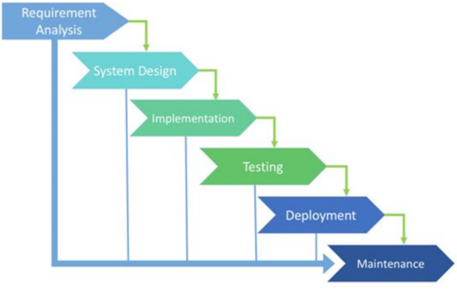
\includegraphics{images/sdlc.png}
    \caption{Software Development Life Cycle Model \cite{SDLC}}
    \label{fig:SDLC}
\end{figure}

\subsection{SAST - Static Application Security Testing}
Expanding on the white-box technique, most vulnerabilities are due to developer's lack of awareness and/or bad programming practices \cite{SAST_opensource} in such a way that \citeauthor{owasp-devsecops-sast} \cite{owasp-devsecops-sast} defines it ``as part of a Code Review'', a ``method of computer program debugging that is done by examining the code without executing the program'', and also a good technic to help find:
    \begin{itemize}
        \item ``Syntax violations''
        \item ``Security vulnerabilities''
        \item ``Programming errors''
        \item ``Coding standard violations''
        \item ``Undefined values''
    \end{itemize}

\subsubsection{Symbolic Execution}
Inside \acrshort{sast}'s set of technics, introduced by \cite{King1976}, we find symbolic execution engines which can help protect systems that range from modern \acrfull{soc} designs and hardware Trojans \cite{Vafaei2021}, to binary-level security analysis such as malware comprehension \cite{David2016} and even a symbiosis between symbolic and concrete execution \cite{Gritti2020}.
All these tools share a common requirement: any instruction set ranging between machine code to source code. These tools excel by mimicking the execution of the analysed software, controlling each value the input influences in the form of symbolic values or variables.

However, a more in-depth look at symbolic execution unveils some obstacles, such as path explosion, constraint solving, environment modelling and others. These symbolic values are allowed to be anything at a first stage, and its value is deciphered further down in the execution path, reducing the possibilities at every branch the execution encounters. The branching happens after performing constraint solving, a very time expensive operation especially when the tested source is of high complexity \cite{Zhang2022}. 

Constraint solving occurs at every moment where a variable value impacts the flow of execution or even once a symbolic variable takes part in any arithmetic computation. This escalates once these computations become of a non-linear nature, such as non-linear expressions and non-linear floating-point computations \cite{Kroening2008}.

Path explosion is one concern found in many high performance problems: the input is sufficiently complex for any sort of resource - be it time, memory, or even processing capacity - to escalate tremendously and becoming unreasonable in a standard environment. When it comes to symbolic execution, a new path is encountered every time a constraint is solved; from that point on, that constraint is a path condition. To better understand this concept, here's an example using the tool \textit{KLEE} according to \cite[p. 3]{Cadar2008}: 
\begin{quote}
``When KLEE detects an error or when a path reaches an exit call, KLEE solves the current path's constraints (called its path condition) to produce a test case that will follow the same path when rerun on an unmodified version of the checked program (e.g., compiled with gcc).''
\end{quote}

Environment modelling is another very common problem in software analysis techniques given how much software development relies on third-party libraries today. This problem escalates whenever these dependencies are packaged as binaries, or the sources are `super-optimized', the paths exploration and consequently the constraint solving may fail which may result in false positives or false negatives \cite{Cadar2008}.
\vfill

\subsection{DAST - Dynamic Application Security Testing} 

The black-box method of testing is very tightly coupled with a hacker perspective of the application; the intention is to find design and/or implementation flaws that cause the system to break down or allow its security to be compromised. Sometimes, to be able to do this a better understanding of the code is required and the testers will frequently find themselves trying to understand how the application is coded.
This technique is known for its low false positive rates, its language independent nature and its ability to detect configuration related attacks. The abstraction of the software implementation is possible because \acrshort{dast} tools require a runtime test case, this means that in the \gls{sdlc} this is applied in the later stages (shift-right) \cite{DAST_description}.

\subsubsection{Fuzzing}
One way to dynamically test software is through fuzzing techniques; this consists of feeding random input with the objective of breaking the application logic or even its execution. \cite{Godefroid2020} also describes it as ``test generation and execution with the goal of finding security vulnerabilities''. Although \textit{fuzzing} is a quick technique, it generally has poor path coverage on its own.

\subsubsection{Dynamic Taint Analysis}
\cite{Schwartz2010} explain that dynamic taint analysis also operates in running programs, but this time by carefully analysing application inputs and each operation to keep track of new and derived taint in an attempt to prevent execution of potentially harmful instructions. Usually, a tainted variable is influenced by user input and then every other variable that is influenced by the first. This technique can be summarized in three steps or \textit{taint policies}: taint introduction, propagation, and checking.

All variables are considered untainted and that only changes when raw user input is stored in one of them, then it becomes a tainted variable. Following user input comes application logic, the same logic that through expressions will contaminate any other variable that interacts with the first set that was tainted by user input. However, once the application gets to a critical operation, it can decide on performing it or not based on how tainted critical variables are  (taint checking).

\subsection{Symbolic Execution}

This work is focused on the static method of application security testing, symbolic execution, and as such we will analyse some available tools. One rather large collection of tools, papers, courses and videos on this thematic is the GitHub repository {ksluckow/awesome-symbolic-execution}%\citetitle{Luckow2017}
 \cite{Luckow2017}.

\subsubsection{Symbolic Execution Engines}\label{subsection:symbolic_exec_engines}

This chapter goes through a selection of engines that were considered for this study: \acrlong{spf}, Jalangi2, SymJS, Cloud9, Kite, KLEE, and Owi. These aren't necessarily better or worse then others that aren't explicitly mentioned. The selection was focused on two characteristics: wide language support and impact on Web Applications. 

Cloud9, Kite, and KLEE, are tools designed, directly or indirectly, for LLVM which supports many different languages \cite{llvm}. Owi is in itself a toolchain designed to improve the \acrshort{wasm} developer experience that also packages a symbolic interpreter for \acrlong{wasm}.


\newcommand{\setool}[1]{\noindent{\large\textbf{\textit{#1}}}\par}

\setool{\acrfull{spf}}
\acrlong{spf} is an extension for the \acrfull{jpf}, a `model checking framework for Java\textsuperscript{TM} bytecode programs' \cite{spf,jpf_wiki}. \acrshort{spf} allows symbolic execution on methods with arguments of basic types, strings, arrays and data structures \cite{spf}.

\setool{Jalangi2}
Jalangi2 is a framework for analysis of JavaScript programs. Jalangi2 was designed to work on browser applications and supports analysis that track `NaNs' or even a memory-profiler but also allows customization through implementation of custom analysis \cite{jalangi2}.

\setool{SymJS}
To test JavaScript web applications there is also SymJS, packed with a symbolic execution engine and also `an automatic event explorer for Web pages'. It is also possible to produce test cases and improve execution through dynamic feedbacks \cite{Li2014}. SymJS references were only found in articles without distributions of software of any kind.

\setool{Cloud9}
Cloud9 was designed with the intent of reducing the `resource-intensive ... nature of high-quality software testing', and claims to be `the first symbolic execution engine that scales to large clusters of machines' \cite{cloud9}. Unfortunately, no source code or executable of this tool was found, the only available link on their homepage wasn't valid.

\setool{Kite}
Kite is a Proof-of-Concept tool that tackles the symbolic execution problem using the \acrfull{cdse} algorithm which is able to dynamically reduce path exploration and is also capable of learning from earlier conflicts \cite{cdse_kite}. Similarly to Cloud9, no source or executable was found and the available links were invalid \cite{kite_web}.

% \hline

\setool{KLEE}
KLEE is perhaps the most relevant tool to address in the LLVM field considering how both Kite and Cloud9 were developed on top of the work acomplished by KLEE. Contrary to what we've seen in the other two tools, KLEE counts with a large community and many papers discussing this tool, its capabilities and other work around it. This is one of our selections for this comparison and more information on it will be presented in \cref{section:klee}.

\setool{Owi}
Owi seems to be the only tool explicitly focused on the \acrlong{wasm} binary format in the list aggregated by \citeauthor{Luckow2017} \cite{Luckow2017}. Nevertheless, it presents promising work specially by their attempt to integrate with the \acrshort{wasm} developer lifecycle with subcommands that allow for other features useful for the everyday tasks like formatting of files and validation of modules \cite{owi_gh}. These and many more features including symbolic execution will be discussed in \cref{section:owi} as this is the second choice for comparison.

\section{SYMBOLIC EXECUTION TOOLS}\label{chap:symbolic_execution_tools}

There are a couple of tools available that perform symbolic execution in numerous ways with different focus and strengths. A good agglomerate of these tools is maintained in a GitHub repository owned by \citeauthor{Luckow2017} \cite{Luckow2017}. There we find symbolic execution tools focused on binaries and various programming languages like Java, JavaScript, or even Rust, but also portable platforms like \glsxtrshort{wasm} and LLVM.

This chapter focuses on the tools that were considered for this work, and the reasons behind the final choice (\cref{section:engines_availability}). Then, the chosen tools, KLEE and Owi, are described in more detail. For both tools, installation instructions, features, and usage examples are provided (\cref{section:klee,section:owi}, respectively). Finally, a comparison between both tools is presented in \cref{section:feat_comp}.

\subsection{Engines Availability}\label{section:engines_availability}

In the endeavour of searching for tools capable of symbolic execution many attempts to have a functional installation of the available alternatives were done, but not all were successfull.

Despite of Cloud9 and Kite having their own websites \cite{cloud9,kite_web} both did not contain valid hyperlinks for either sources or a compiled binary of the software. On the other hand, for SymJS nothing more than a scientific document was found \cite{Li2014}.

That leaves us to KLEE and Owi, a pair of tools with a large support of languages \cite{llvm,wasm_fermyon}, and \glsxtrshort{spf} and Jalangi2, the two programming languages used to develop the WebGoat project maintained by \glsxtrshort{owasp} \cite{webgoat,owasp_webgoat}. \glsxtrshort{owasp} WebGoat project is an intentionally vulnerable application so developers interested in learning cybersecurity can use it to learn about vulnerabilities \cite{owasp_webgoat}.

Despite the interest around \glsxtrshort{owasp}'s WebGoat project and the availability of sources for both \glsxtrshort{spf} and Jalangi2, getting each software to run on their own and consistently is a daunting task with not much documentation to go along and a steep learning curve.

KLEE and Owi are both far better when it comes to the available documentation, and initial learning curve; the users are not bombarded with a codebase and a single `README' file, instead they have either multiple README's for each subcommand \cite{owi_gh} or a large number of papers and websites with tutorials, examples and information on the tool features \cite{Cadar2008,ADALogicsKLEE,klee_tutorial1,klee_tutorial2,klee_install}.

 
Given the current software paradigm, where performance is important not only in the matter of software runtime but also when it comes to software development, maintenance, and portability, tools that apply to technologies such as LLVM and WASM are interesting research targets.
Therefore, we are looking at KLEE and Owi, which propose solutions for each tech stack, respectively.

\subsection{KLEE}\label{section:klee}

KLEE explores the LLVM infrastructure rather successfully and with speed; however, this engine bottlenecks quite considerably when it is applied on larger scale projects. This is due to its space management, given how it tries to keep all relevant information about the current states. It is also unable to handle dynamically generated code, concurrent execution and struggles with modelling network and peripherals, although most peers share these weaknesses \cite{NSabinoSymbolicExecution}. The LLVM project supports many different languages like Haskell, Rust and Python, but our test cases will focus on C/C++ programs \cite{llvm}.
.

LLVM has been referenced a few times in this document, but a brief explanation is in order. LLVM is not an acronym, but the full name of the project. Despite the name, it has nothing to do with virtual machines. LLVM is ``a collection of modular and reusable compiler and toolchain technologies''. It is also praised for its versatility, flexibility, and reusability. For more information about LLVM, please refer to their website \cite{llvm}.

\cite{Cadar2008} describe KLEE as being in both static and dynamic techniques of testing: every symbolic execution engine is static by definition, but KLEE becomes dynamic through its outside environment interaction features.

% \vfill5
% \subsubsection{Installation}\label{section:klee_install}

% The KLEE \acrshort{cli} tool is available in many ways and one of the fastest ways to get started is through their Docker image, but they also publish to the Snap Store and many package managers. However, the KLEE authors recommend building from source.

% A manual installation is demanding immediately from the dependencies' installation - 16 packages are required to install KLEE, 2 of which are optional (to generate documentation), and 3 more are recommended for improved usability. All the required commands are available in the \Cref{lst:klee_dependencies}.

% \noindent % avoid overflow
% \begin{minipage}{\textwidth}
% \begin{lstlisting}[
% boxpos={ht},
% caption={KLEE dependencies installation.},
% label={lst:klee_dependencies},
% ]
% # graphviz/doxygen are optional (documentation generation)
% sudo apt-get install build-essential cmake curl file \
%     g++-multilib gcc-multilib git libcap-dev \
%     libgoogle-perftools-dev libncurses5-dev libsqlite3-dev \
%     libtcmalloc-minimal4 python3-pip unzip graphviz doxygen

% # additional features in `klee-stats'
% sudo apt-get install python3-tabulate

% # `lit' enables testing 
% # `wllvm' makes it easier to compile to LLVM bitcode
% sudo apt-get install pipx
% pipx install lit wllvm

% \end{lstlisting}
% \end{minipage}

% Base dependencies aside, KLEE still requires critical tools such as LLVM 13 and at least one constraint solver; KLEE was built on top of LLVM 13 and the STP solver tools, but also supports Z3. LLVM 13 and the STP solver can be installed by using the commands in \Cref{lst:klee_llvm_install,lst:klee_stp_dependencies,lst:klee_stp_install}.

% \begin{lstlisting}[
% boxpos={ht},
% caption={LLVM installation.},
% label={lst:klee_llvm_install},
% breaklines=true,
% postbreak=\mbox{\textcolor{red}{$\hookrightarrow$}\space},
% ]
% # add LLVM repositories to `apt' package manager
% wget -O - https://apt.llvm.org/llvm-snapshot.gpg.key | sudo apt-key add -

% # install LLVM packages
% sudo apt-get install clang-13 llvm-13 llvm-13-dev llvm-13-tools
% \end{lstlisting}

% \begin{lstlisting}[
% boxpos={ht},
% caption={STP dependencies installation.},
% label={lst:klee_stp_dependencies},
% breaklines=true,
% postbreak=\mbox{\textcolor{red}{$\hookrightarrow$}\space},
% ]
% # STP dependencies
% sudo apt-get install cmake bison flex libboost-all-dev python perl zlib1g-dev minisat

% # clone MiniSAT
% git clone https://github.com/stp/minisat.git
% cd minisat

% # build
% mkdir build
% cd build
% cmake -DCMAKE_INSTALL_PREFIX=/usr/local/ ../

% # install
% sudo make install
% \end{lstlisting}

% \noindent
% \begin{minipage}{\textwidth}
% \begin{lstlisting}[
% boxpos={ht},
% caption={STP installation.},
% label={lst:klee_stp_install},
% breaklines=true,
% postbreak=\mbox{\textcolor{red}{$\hookrightarrow$}\space},
% ]
% # clone STP
% git clone https://github.com/stp/stp.git
% cd stp
% git checkout tags/2.3.3

% # build
% mkdir build
% cd build
% cmake ..
% make

% # install
% sudo make install

% # increase stack size to run KLEE on larger benchmarks
% ulimit -s unlimited
% \end{lstlisting}
% \end{minipage}

\subsubsection{Features}

KLEE is packaged with multiple \glsxtrshort{cli}s (see \Cref{tab:klee_features}) that contribute to the user experience, but the main command that runs the symbolic execution engine is \lstinline{klee}. 

\begin{table}[ht]
    \begin{center}
    \begin{tabular}{r|l}
    \multicolumn{1}{c|}{Command} & \multicolumn{1}{c}{Description} \\
    \hline
    \hline
    \lstinline$kleaver$ & Operates on \lstinline$.kquery$ files. \\
    \lstinline$klee-exec-tree$ & Takes \lstinline$klee$ tree output and displays a graphical \\&representation or statistics.\\
    \lstinline$klee-replay$ & Takes one ktest from a file or multiple from a \\&directory and runs them. \\
    \lstinline$klee-stats$ & Takes \lstinline$klee$ stats output and processes it as \\&instructed. \\
    \lstinline$klee-zesti$ & \glsxtrshort{zesti}\textsuperscript{1} like wrapper of KLEE. \\
    \lstinline$ktest-gen$ & Generates test cases (a \lstinline$.ktest$ file) from \\&concrete input. \\
    \lstinline$ktest-randgen$ & Generates test cases (a \lstinline$.ktest$ file) from \\&randomly generated input. \\
    \lstinline$ktest-tool$ & Describes a \lstinline$.ktest$ file containing information \\&on each input object. \\
    \multicolumn{2}{l}{\textsuperscript{1}\glsxtrfull{zesti}}
    \end{tabular}
    \caption{KLEE commands.}
    \label{tab:klee_features}
    \end{center}
\end{table}

\subsubsection{Instrumentation}\label{subsection:klee_instrumentation}

The KLEE web page contains a tutorials section to help get familiarized with the tool. These tutorials contain samples and instructions on how to properly set up a C/C++ source file, let's call it code instrumentation, and how to run and analyse the results. Their sources can be found in higher detail in appendix \ref{appendix:klee}.

The first, and most basic example, shows how one can mark a variable as symbolic by using the \lstinline$klee_make_symbolic()$ function (see \Cref{lst:klee_instrumentation}). This function takes 3 arguments; the first two will define a memory range in which the variable information is stored, the third defines a human-readable object name that identifies the symbolic variable in the generated test case files (for the variable `\lstinline$a$' declared on \cref{var:klee_instrumentation_var_a} in \Cref{lst:klee_instrumentation}, this could be ``my variable''.):

\begin{enumerate}
    \item The variable memory address,
    \item The variable memory size,
    \item The variable name, a human-readable identifier.
\end{enumerate}

Running \lstinline$klee$ on the compiled LLVM bitcode did not return any error but does return a couple of other interesting details. On \cref{line:complete_paths,line:partial_paths,line:generated_tests} of the \Cref{lst:klee_instrumentation_output}, we have information on the number of completely and partially complete traced paths, and lastly the number of generated test cases. Every traced path has a corresponding test, but only detected errors generate error information and an error query; these two different informations will be covered later once we start looking at test examples on \cref{chap:experiences} \nameref{chap:experiences}.

\lstinputlisting[
% boxpos=ht,
caption={Tutorial 1 \lstinline$klee$ output},
label={lst:klee_instrumentation_output},
escapechar=|,
numbers=left,
breaklines=true,
postbreak=\mbox{\textcolor{red}{$\hookrightarrow$}\space},
]{code-snippets/chap3/klee_instrumentation_output}

% minipage maybe
% \noindent\begin{minipage}{\linewidth}
\lstinputlisting[
% boxpos=ht,
language=C,
caption={Tutorial 1 sample},
label={lst:klee_instrumentation},
escapechar=|,
numbers=left,
]{code-snippets/chap3/klee_instrumentation}
% \end{minipage}

Another valuable feature, is the \lstinline$klee_prefer_cex()$ that tells KLEE to prefer a set of values when generating test cases; this allows the user to get readable results like ``aaaa'' instead of hexadecimal representation of character values such as ``\textbackslash xff\textbackslash xff\textbackslash xff\textbackslash xff''.

\subsubsection{Running KLEE}\label{subsection:running_klee}

% To properly analyse a program's execution using KLEE, there are some requirements in order for it to work as expected. KLEE needs to be told essential information about the software, like what variables are classified as inputs and even what interval of values they are known to be constrained. This is possible using the functions available in the KLEE library (\lstinline{#include <klee/klee.h>}) such as \lstinline{klee_make_symbolic()} and \lstinline{klee_assume()}.

After instrumenting the source code with KLEE instructions, see \cref{subsection:klee_instrumentation}, the next step is compiling it to LLVM, and the easiest way to achieve that is using Clang (\Cref{lst:klee_clang}).

\begin{lstlisting}[
caption={Basic clang command},
label={lst:klee_clang}
]
clang -emit-llvm -c main.c
\end{lstlisting}

When compiling programs that include the klee library, it may be needed to include the klee library, so Clang understands its instructions, which can be done like in \Cref{lst:klee_clang_with_lib}.

\begin{lstlisting}[
caption={Basic clang command with path to klee library},
label={lst:klee_clang_with_lib}
]
clang -I $PATH_TO_KLEE_LIBRARY -emit-llvm -c main.c
\end{lstlisting}

However, the KLEE documentation recommends a more complete command to have access to a more complete set of functionality that klee provides, such as test replayability, and that command is available in \Cref{lst:clang-complete}.

\begin{lstlisting}[
caption={Complete clang command},
label={lst:clang-complete}
]
clang -emit-llvm -c -g -O0 -Xclang -disable-O0-optnone main.c
\end{lstlisting}

The compilation command should return an object with extension `$.bc$' containing the LLVM representation of the program. This file is in the correct format for KLEE, and therefore we can now test it by running the command on \Cref{lst:klee_run_example}.

\begin{lstlisting}[
caption={Running klee on a program},
label={lst:klee_run_example}
]
klee main.bc
\end{lstlisting}

Running KLEE on a program results in file outputs, the \lstinline$klee-out-n$ and \lstinline$klee-last$ folders are created. For \lstinline$klee-out-n$, \lstinline$n$ is the zero-indexed counter of the run, and \lstinline$klee-last$ is a symbolic link to the most recent run folder; by the second run of KLEE, \lstinline$klee-last$ points to \lstinline$klee-out-1$. The folders created by KLEE contain all the generated test cases, error reports, and other useful information about the execution. Each generated test case is stored in a file with extension `$.ktest$' and can be analysed using the \lstinline$ktest-tool$ command (see \Cref{lst:klee_ktest_tool}).

\begin{lstlisting}[
caption={Analyzing a ktest file},
label={lst:klee_ktest_tool}
]
$ ktest-tool klee-last/test000001.ktest
ktest file : 'klee/klee-last/test000001.ktest'
args       : ['main.bc']
num objects: 1
object 0: name: 'my signed integer'
object 0: size: 4
object 0: data: b'\x00\x00\x00\x00'
object 0: hex : 0x00000000
object 0: int : 0
object 0: uint: 0
object 0: text: ....
\end{lstlisting}

% \section{Symbolic Execution Tools}

\subsection{Owi}\label{section:owi}

Reference \cite{Andrès2024} describes Owi as a toolkit that aggregates functionality to assist WebAssembly developers, one of which enables the compilation of C code to \glsxtrshort{wasm} and running their symbolic interpreter on top of it.

\glsxtrlong{wasm} is a portable binary instruction format for executable programs, designed to be a compilation target for high-level languages like C/C++ and Rust, enabling deployment on the web for client and server applications. WebAssembly is designed to be fast, efficient, and secure, making it an ideal choice for running complex applications in web browsers and other environments \cite{wasm_home,wasm_use_cases}.

% \subsubsection{Installation}

% To properly make use of the tool, a working installation is required and Owi is officially available in two ways. The first and more direct approach is by using the opam, the OCaml Package Manager. The second alternative is through a manual installation using $dune$, the OCaml build system, which can also be installed using $opam$ or manually using $make$ commands.

% The first method resulted in an unusable binary (when it comes to symbolic execution), without any helpful information or help page when running it, therefore is recommendable the use of the second method and building the tool from the repository yourself. To do so, all that needs to be done is running the instructions in \Cref{lst:owi_install} to install \lstinline+opam+, the required dependencies, which include \lstinline+dune+, and finally building and installing \lstinline+owi+.

% \begin{lstlisting}[
% boxpos={ht},
% caption={Owi installation},
% label={lst:owi_install},
% language=bash
% ]
% # install opam 
% apt install opam
% # install owi dependencies
% opam install . --deps-only
% # build owi
% dune build -p owi @install
% # install owi
% dune install
% \end{lstlisting}

\subsubsection{Features}

Owi being a toolchain designed for the development of \glsxtrshort{wasm}, it provides a set of subcommands as listed in \Cref{tab:owi_features}; however, to be able to use the symbolic interpreter packaged with it, we need to also install a restraint solver. Owi supports any Smt.ml supported solver, but the default solver is Z3.

Owi also supports test replayability from an output file generated by the $sym$ subcommand as you can see in \Cref{lst:owi_replay}.

\begin{lstlisting}[
boxpos={ht},
caption={Owi replayability model},
label={lst:owi_replay},
language=bash
]
owi sym main.wat > main.model
owi replay --replay-file=main.model main.wat
\end{lstlisting}

\begin{table}[ht]
    \centering
    \begin{tabular}{r|l}
    \multicolumn{1}{c|}{Subcommand} & \multicolumn{1}{c}{Description} \\
    \hline
    \hline
    $c$ & Compiles C source code to \glsxtrshort{wasm} and runs the \\&\glsxtrshort{wasm} symbolic interpreter on the end result. \\
    $conc$ & Takes \glsxtrshort{wasm} input and runs the concolic interpreter \\&on it.\\
    $fmt$ & Formats \glsxtrlong{wasm} text format files ($.wat$ or \\&$.wast$).\\
    $opt$ & Optimizes \glsxtrlong{wasm} modules.\\
    $run$ & Runs the concrete interpreter.\\
    $replay$ & Replay a \glsxtrshort{wasm} module containing symbols with \\&concrete values in a replay file containing a model.\\
    $script$ & Runs a reference test suite script.\\
    $sym$ & Takes \glsxtrshort{wasm} input and runs the symbolic interpreter \\&on it.\\
    $validate$ & Validates \glsxtrlong{wasm} modules.\\
    $wasm2wat$ & Generate a text format file ($.wat$) from a binary \\&format file ($.wasm$).\\
    $wat2wasm$ & Generate a binary format file ($.wasm$) from a text \\&format file ($.wat$).\\
    \end{tabular}
    \caption{Owi subcommands}
    \label{tab:owi_features}
\end{table}

\subsubsection{Instrumentation}\label{subsection:owi_instrumentation}

The Owi repository maintains a folder with examples of how to use the different subcommands; similarly to KLEE, we have available multiple examples on how to use \lstinline$owi c$ that are detailed in appendix \ref{appendix:owi}.

Looking at the first example, some differences from KLEE are evident, specifically how the tool is informed about which variables are symbolic. KLEE uses the variable address and the type is disregarded in the whole process (the generated test cases detail values for each possible primitive type); Owi on the other hand expects to be told the symbolic variable type, through the available functions:

% \parbox{\textwidth}{
\begin{itemize}
    \item \lstinline$owi_i32()$ - to define 32-bit integer values, with 8-bit and 64-bit variants;
    \item \lstinline$owi_f32()$ - to define 32-bit floating-point values, with a 64-bit variant;
    \item \lstinline$owi_char()$ - to define character values;
    \item \lstinline$owi_bool()$ - to define boolean values.
\end{itemize}
% }

Unlike KLEE functions, these do not support any argument that allows defining a custom name for the symbolic variable; the symbols are identified by order of creation - if we define all positions of an array as symbolic, each position symbolic identifier would correspond to their array position, but if any other symbol is defined before the identifiers would shift by the number of predefined variables.

To run Owi on a simple sample we must include the Owi library in the source code so it is possible to find Owi function implementations and generate a valid WebAssembly module. As visible on \Cref{lst:owi_instrumentation}, the variable \lstinline$x$ of type \lstinline$int$ is instrumented using the routine \lstinline$owi_i32$ (\cref{line:owi_var_x}) and since this program is trying to find the roots of a polynomial, we want the symbolic values that result in \lstinline$poly == 0$, therefore \cref{line:owi_assert_poly} will catch a `problem' every time \lstinline$poly$ equals 0 since the passed condition evaluates to \lstinline$false$.

There are in fact solutions to the defined polynomial and Owi outputs them as visible in \Cref{lst:owi_instrumentation_output}. The output represents a test case, and to replicate the test case one or more of the passed inputs must have a specific set of values. On the example at hand, only one symbol was defined and its state is displayed on \cref{line:owi_symbol_0}. The second value on this line is the symbols' name (\lstinline$symbol_0$), then follows the symbol's type and since an integer was defined its type \lstinline$i32$. Finally, its value is also presented, in this case we can state that 4 is one solution to the polynomial written on \Cref{lst:owi_instrumentation}.

Owi also produces a \lstinline$owi-out/test-suite$ folder and inside it a \lstinline$testcase-N.xml$, where \lstinline$N$ is an index starting on 1, that describes the input value for a symbolic variable for that test case, and a \lstinline$metadata.xml$ that details the arguments of the owi executation such as the source code language, which Owi subcommand produced the file, the input program file (`\textit{poly.c}') and other details on the execution. The generated test cases are relevant to found issues, Owi does not generate test cases on each traced path like KLEE does.

% \noindent\begin{minipage}{\linewidth}
\lstinputlisting[
boxpos=ht,
caption={Polynomial example 1 source code with Owi instrumentation},
label={lst:owi_instrumentation},
escapechar=|,
numbers=left,
escapechar=|,
breaklines=true,
% upquote=true,
showstringspaces=false,
postbreak=\mbox{\textcolor{red}{$\hookrightarrow$}\space},
]{code-snippets/chap3/owi_instrumentation}
% \end{minipage}

\lstinputlisting[
boxpos=ht,
caption={Polynomial example 1 output},
label={lst:owi_instrumentation_output},
escapechar=|,
numbers=left,
escapechar=|,
breaklines=true,
% upquote=true,
showstringspaces=false,
postbreak=\mbox{\textcolor{red}{$\hookrightarrow$}\space},
]{code-snippets/chap3/owi_instrumentation_output}

\subsubsection{Running Owi}

Similarly to KLEE, Owi provides a set of methods to inform the symbolic interpreter in an attempt to improve the results, examples of this are \lstinline{owi_assume()} and \lstinline{owi_i32()} for int32 variables (and others for the respective primitive types such as \lstinline{owi_char()}).

Once the sources are ready, running the symbolic interpreter is very simple with Owi by running \autoref{lst:owi-command}. Since this is a toolkit it contains many subcommands, the most relevant for this study being the `$c$' subcommand that allows running C code directly.

\begin{lstlisting}[
caption={Running owi on a program source.},
label={lst:owi-command}
]
owi c main.c
\end{lstlisting}

However, if your program requires any sort of custom option or if you just want to experiment with them, we can `ask' Owi how they compile the sources. To do that, all one needs to do is run \lstinline$owi c main.c --debug$ on invalid C files and will find in the tool output the command in \Cref{lst:owi_clang}.

% \noindent\begin{minipage}{\linewidth}
\begin{lstlisting}[
boxpos=ht,
caption={Owi abstracted compilation command (clang).},
label={lst:owi_clang},
breaklines=true,
escapechar=|,
]
clang -O3 --target=wasm32 -m32 -ffreestanding \
    |\mbox{\textcolor{red}{$\hookrightarrow$}\space}|--no-standard-libraries -Wno-everything -flto=thin \
    |\mbox{\textcolor{red}{$\hookrightarrow$}\space}|-Wl,--entry=main -Wl,--export=main -Wl,--lto-O0 \
    |\mbox{\textcolor{red}{$\hookrightarrow$}\space}|-Wl,-z,stack-size=8388608 \
    |\mbox{\textcolor{red}{$\hookrightarrow$}\space}|-I $HOME/.opam/default/share/owi/libc -o main.wasm \ 
    |\mbox{\textcolor{red}{$\hookrightarrow$}\space}|$HOME/.opam/default/share/owi/binc/libc.wasm \
    |\mbox{\textcolor{red}{$\hookrightarrow$}\space}|main.c
\end{lstlisting}
% \end{minipage}

Owi also integrates Frama-C's E-ACSL plugin. This plugin enables the detection of implementation issues, or even custom heuristics for complex bugs, through the definition of a set of rules that can create constraints on acceptable inputs (`requires') and outputs (`ensures'). The \lstinline$owi c$ subcommand and to enable all one needs to do is pass the argument \lstinline$--e-acsl$. To see how Frama-C is being executed the process is similar as to the compilation, but now with the E-ACSL option, and it looks like \Cref{lst:owi_frama_c}. This plugin enables the detection of implementation issues, or even custom heuristics for complex bugs, through the definition of a set of rules that can create constraints on acceptable inputs (`requires') and outputs (`ensures').

\begin{lstlisting}[
boxpos=ht,
caption={Owi abstracted Frama-C instrumentation of E-ACSL.},
label={lst:owi_frama_c},
breaklines=true,
escapechar=|,
% upquote=true,
showstringspaces=false,
]
frama-c -e-acsl -no-frama-c-stdlib \
    |\mbox{\textcolor{red}{$\hookrightarrow$}\space}|-kernel-warn-key CERT:MSC:38=inactive -verbose 2 \
    |\mbox{\textcolor{red}{$\hookrightarrow$}\space}|-cpp-extra-args="-I$HOME/.opam/default/share/owi/libc" \
    |\mbox{\textcolor{red}{$\hookrightarrow$}\space}|main.c -then-last -print -ocode main.instrumented.c
\end{lstlisting}

After compiling either \lstinline$main.c$ or \lstinline$main.instrumented.c$, the resulting \lstinline$.wasm$ object can be tested with Owi using the command on \Cref{lst:owi-sym-command}.

\begin{lstlisting}[
caption={Running owi on a compiled program.},
label={lst:owi-sym-command},
]
owi sym main.wasm
\end{lstlisting}

Executing either \lstinline$c$ or \lstinline$sym$ subcommands generates some files inside the folder `owi-out' created on the current working directory: \lstinline$owi sym$ only generates test case files named `testcase-n.xml' being $n$ the number of results detected and starting from 1. The subcommand \lstinline$owi c$ also generates a file describing the test cases that fail execution, but also outputs an additional `metadata.xml' 
% as described in \Cref{tab:owi_c_owi_out}
, and a `a.out.wasm' file (the compiled sources); however, the test case and metadata files are generated in a subfolder called `test-suite' while the \glsxtrlong{wasm} module is created on the current working directory (at the same level as `owi-out' folder).
For a visual reference of this file structure take a look at \Cref{lst:owi-generated-files}, consider `main.c' the input sources and `main.wasm' pre-compiled before running Owi.

% \begin{table}[ht]
%     \centering
%     \begin{tabular}{r|c|l}
%         \multicolumn{1}{c|}{Field} & \multicolumn{1}{c|}{Example} &\multicolumn{1}{c}{Description} \\
%         \hline
%         \hline
%         \lstinline$sourcecodelang$ & `C' & The programming language in \\&&which the input sources are \\&&written \\
%         \lstinline$producer$ & `owic' & The subcommand responsible for \\&&this metadata file.\\
%         \lstinline$specification$ & N/A & \multicolumn{1}{c}{No information on this}\\&& \multicolumn{1}{c}{field was found}\\
%         \lstinline$programfile$ & `main.c' & The input source files\\
%         \lstinline$programhash$ & b663247... & The compiled wasm module hash\\
%         \lstinline$entryfunction$ & `main' & \glsxtrshort{wasm} modules requires by \\&&default a specific entry point, \\&&in this case Owi defines `main'\\
%         \lstinline$architecture$ & `32bit' & The target architecture (defined \\&&by Owi)\\
%         \lstinline$creationtime$ & timestamp & The day and time this metadata \\&&file was created\\
%     \end{tabular}
%     \caption{Owi `metadata.xml' file contents.}
%     \label{tab:owi_c_owi_out}
% \end{table}

\noindent
% \begin{minipage}{\textwidth}
\begin{lstlisting}[
caption={Owi generated files structure.},
label={lst:owi-generated-files},
literate={├}{{\textSFviii}}1 {─}{{\textSFx}}1 {└}{{\textSFii}}1 {│}{{\textSFxi}}1,
]
# owi c ...
.
├── a.out.wasm
├── main.c
└── owi-out
   └── test-suite
      ├── metadata.xml
      └── testcase-1.xml

# owi sym ...
.
├── main.c
├── main.wasm 
└── owi-out
   └── testcase-1.xml
\end{lstlisting}
% \end{minipage}

\subsection{Feature Comparison}\label{section:feat_comp}

Not only it is important to understand how well a tool performs, but also how flexible it can be in the different scenarios it may face. \Cref{tab:feature_comparison} summarizes the comparison, and is divided into 3 sections. %\Cref{tab:feature_comparison} was built describing each tool supported vulnerabilities, their ease-of-use, how easy they are to install, and which STP solvers they support. The tools' installation speed and complexity are scaled from 1-5 ranging from very slow to very fast or very hard to very easy, respectively. The third and fourth columns (Ease-of-use for beginner and experienced developers) take the same scale as the second one: 1-5, very hard to very easy.

% The tools' installation process is very different both in the amount of methods but also in the complexity of the provided solutions. Although the recomended solution by \citeauthor{klee_install} \cite{klee_install} is very complex since it requires a lot of dependencies and different processes, 
% % as we discussed in \cref{section:klee_install},
% there is also available a quick start option using a docker image made available by the maintainers of KLEE. In contrast, Owi does not offer many ways to install its engine but both of them require the installation of \lstinline$opam$ but also \lstinline$dune$ if one compiles the source code directly. 

% With their differences in mind, KLEE punctuates a score of 5 in installation speed but if we disregard the Docker approach, both KLEE and Owi take 2 points; even though the first requires much more commands and dependencies, the second takes more time to actually compile the repository.

% When it comes to installation complexity, KLEE clearly could use some improvement in build automatization while Owi leverages this quite well with \lstinline$opam$ and \lstinline$dune$ however these are tools very tied with OCaml development which is not at all the focus of this study adding unnecessary complexity to the installation process. Considering this, KLEE scores a 1 in the recommended process. But if using Docker is an option, then it scores a 4. Owi on the other hand scores a 3, much because of the OCaml tools; we're intentionally ignoring the opam package since it did not produce a valid installation, otherwise Owi could score a 5.

% The tools usability is also scored in the perspective of both beginners and experienced developers. Because KLEE has so much documentation available across the internet the learning curve is very stable but the more advanced the requirements the more complex the usage may get due to how some functionalities are scattered across different \glsxtrshort {cli}'s, these two points contribute for a solid positive score (4). Owi on the other hand can pose as a hard obstacle for the least experienced mainly due to the lack of support documents and the fact that OCaml doesn't make it into the top 50 of most popular programming languages where the 50th most popular language rates 0.15\%, according to \citeauthor{tiobe_index}\cite{tiobe_index}, scoring 2 points in this scenario. The popularity issues become nearly non-existent when an experienced mind makes use of the tool and the simplicity of having all tools aggregated into one \glsxtrshort {cli} also contributes to a better score (4).

The first section of \Cref{tab:feature_comparison} describes the installation process and ease-of-use of each tool. Installation is scored in two dimensions: speed and complexity. KLEE supports a quick start using Docker, which is very fast to set up but may not be the best option for everyone. The recommended installation process is more complex and time-consuming, which is reflected in the scores. Owi doesn't offer a docker image. 

The second section of \Cref{tab:feature_comparison} describes features and heuristics supported by each tool; heuristics refers to software vulnerabilities/errors, if they are supported by the tools and how these heuristics are defined. % This is analysed in higher detail in \cref{chap:experiences}.

% The last section of \Cref{tab:feature_comparison} aggregates information from KLEE and Owi documentation on SAT and SMT solvers. While SAT solvers handle \textit{boolean satisfiability}, SMT expand on this concept into general formulas\cite{rbc_sat_solvers}. Examples of SMT solvers are STP and Z3 but there are also wrappers like MetaSMT and frontends as Smt.ml \cite{stp_solver,z3_solver,metaSMT,smtml}. MiniSat is a SAT solver used by STP as the underlying SAT solver and Smt.ml also has MiniSat in its support roadmap \cite{minisat,smtml}.

The last section of \Cref{tab:feature_comparison} summarizes how KLEE and Owi compare in terms of supporting SAT and SMT solvers. While SAT solvers handle \textit{boolean satisfiability}, SMT expand on this concept into general formulas\cite{rbc_sat_solvers}. After looking at both KLEE and Owi documentation, we can see that KLEE supports more solvers overall.

% Features table
\begin{table}[tb]
    \centering
    \caption{Feature comparison}
    \begin{tabular}{l|c|c}
       \multicolumn{1}{c|}{\textit Feature} & \multicolumn{1}{c|}{KLEE} & \multicolumn{1}{c}{Owi} \\
       \hline
       \hline
        Installation speed & 5 (2) & 2 \\
        Installation complexity & 1 (4) & 3 \\
        Ease-of-use (begginer) & 4 & 2 \\
        Ease-of-use (experienced) & 4 & 4 \\
        \hline
        \hline
        Heuristics support & Larger & Reduced \\
        Heuristics definition & Hardcoded & Hardcoded \\
        Supports E-ACSL & NO & YES \\
        \hline
        \hline
        SAT/SMT solvers support & Larger & Reduced \\
        % Supports MetaSMT & YES & NO \\
        % Supports STP & YES & NO \\
        % Supports Z3 & YES & YES \\
        % Supports metaSMT solvers & YES & NO \\
        % Supports Smt.ml solvers & NO & YES \\
        % Supports MiniSat & YES & NO\\
    \end{tabular}
    \label{tab:feature_comparison}
\end{table}

% \footnotetext[3]{`metaSMT is a wrapper around various SMT or SMT-like solvers.'\\\cite{metaSMT}}
% \footnotetext[4]{`Smt.ml is a Multi Back-end Front-end for SMT Solvers in OCaml.'\\\cite{smtml}}
% \footnotetext[5]{Supported as the underlying SAT solver for STP}
% \footnotetext[6]{Support planned by the Smt.ml maintainers}
\section{EXPERIENCES AND RESULTS}\label{chap:experiences}

In this section, multiple experiences using both KLEE and Owi tools will be described and analysed. We will start by describing the test environment in \cref{section:test_environment}, and then proceed to summarize the experiments ran in \cref{section:test_samples}. The metrics used to evaluate the tools will be presented in \cref{section:metrics}, and finally a summary of all results and an analysis will be presented in \cref{section:results}.
Each experience will showcase their capabilities and limitations. 

\subsection{Test Environment}\label{section:test_environment}

To increase the results' credibility, all tests were run on the same machine, therefore sharing the same resources. The specifications of such machine consisted in a 12th Gen Intel Core processor (i7-1255U) of 10 cores (and a total of 12 threads) with a max clock speed of 4.70 GHz, and 20 GB (4 + 16) of DDR4 3200 MHz RAM. 

This is the parent system setup with a Windows 11 installation; however, the test environment was created in a WSL environment within this machine which shares 4 cores and 8 GB of RAM available.

For simplicity of testing, all samples were organized by folders and subfolders: the parent folder aggregates by sample and child folders aggregates files by tool, KLEE or Owi.

\subsection{Test Samples}\label{section:test_samples}

To compare the tools we will run them in 9 samples. The samples 1 and 2 were extracted from KLEE's online documentation \cite{klee_tutorial1,klee_tutorial2} and samples 3 through 5 from Owi's GitHub repository \cite{owi_gh}. 
Samples 6 through 9 were recovered from \citeauthor{ADALogicsKLEE} blog \cite{ADALogicsKLEE}. All samples were adapted with necessary changes to ensure compatibility with both tools. They cover, in that order, the following vulnerabilities: 

% \citeauthor{ADALogicsKLEE} \cite{ADALogicsKLEE}
%  presents 4 videos to demonstrate KLEE set of features and in video 3 they discuss vulnerabilities of the types:

\begin{itemize}
    \item Global Buffer Overflow
    \item Stack-based Buffer Overflow
    \item NULL pointer dereference
    \item Use after \lstinline$free$
\end{itemize}

We can look at sample 7 as an example of how KLEE and Owi compare. Stack-based Buffer Overflow vulnerabilities look at scoped and dynamically allocated variables like the one on line 8 of \cref{lst:chap4_sample7_test2}. To run KLEE and Owi on this sample, the sources were instrumented as shown on \Cref{lst:chap4_sample7_klee} and \Cref{lst:chap4_sample7_owi}, respectively.

% Running KLEE results in 6 generated tests, one of which triggered an execution error shown in detail on \Cref{lst:chap4_sample7_klee_test}. This time, the error occurs on \cref{line:4_7_error} of file main (\Cref{lst:chap4_sample7_klee}).
% Owi fails to find the vulnerability on this sample.

% \begin{lstlisting}[
% caption={Sample 7 - KLEE output},
% label={lst:chap4_sample7_klee_output},
% % upquote=true,
% escapechar=@,
% numbers=left,
% breaklines=true,
% postbreak=\mbox{\textcolor{red}{$\hookrightarrow$}\space},
% ]
% KLEE: NOTE: KLEE: ERROR: main.c:26: memory error: out of bound pointer
% now ignoring this error at this location

% KLEE: done: total instructions = 12566
% KLEE: done: completed paths = 5
% KLEE: done: partially completed paths = 1
% KLEE: done: generated tests = 6
% \end{lstlisting}

% \begin{lstlisting}[
% caption={Sample 7 - KLEE test case for the detected error},
% label={lst:chap4_sample7_klee_test},
% % upquote=true,
% escapechar=@,
% numbers=left,
% breaklines=true,
% postbreak=\mbox{\textcolor{red}{$\hookrightarrow$}\space},
% ]
% ktest file : './sample7/klee/klee-last/test000003.ktest'
% args       : ['main.bc']
% num objects: 1
% object 0: name: 'arr'
% object 0: size: 10
% object 0: data: b'BUG!\x00\xff\xff\xff\xff\x00'
% object 0: hex : 0x4255472100ffffffff00
% object 0: text: BUG!......
% \end{lstlisting}

\lstinputlisting[
caption={Sample 7 - test2 function code},
label={lst:chap4_sample7_test2},
language=c,
% upquote=true,
numbers=left,
breaklines=true,
showstringspaces=false,
postbreak=\mbox{\textcolor{red}{$\hookrightarrow$}\space},
]{code-snippets/chap4.sample7/function_test2}

\lstinputlisting[
caption={Sample 7 - KLEE instrumentation},
label={lst:chap4_sample7_klee},
language=c,
% upquote=true,
numbers=left,
breaklines=true,
showstringspaces=false,
postbreak=\mbox{\textcolor{red}{$\hookrightarrow$}\space},
]{code-snippets/chap4.sample7/klee_main}

\lstinputlisting[
caption={Sample 7 - Owi instrumentation},
label={lst:chap4_sample7_owi},
language=c,
% upquote=true,
numbers=left,
breaklines=true,
showstringspaces=false,
postbreak=\mbox{\textcolor{red}{$\hookrightarrow$}\space},
]{code-snippets/chap4.sample7/owi_main}

% \subsection{Sample 8 - NULL pointer dereference}\label{section:sample_8}

% To test NULL pointer dereference bugs, a small string array (`\lstinline$char *global_string[]$' on \cref{line:4_8_global_var}) is initialized and used in function `\lstinline$test3$' where on \cref{line:4_8_error} will trigger an error when the input is favorable.

% After the samples are instrumented, the tools are run and a pattern begins to show where KLEE detects the vulnerability but Owi does not. See \Cref{lst:chap4_sample8_klee,lst:chap4_sample8_owi} for KLEE and Owi instrumented samples, respectively, \Cref{lst:chap4_sample8_klee_output} for KLEE terminal output and \Cref{lst:chap4_sample8_klee_test} for the generated test case.

% \lstinputlisting[
% caption={Sample 8 - Owi instrumentation},
% label={lst:chap4_sample8_owi},
% escapechar=@,
% language=c,
% numbers=left,
% breaklines=true,
% postbreak=\mbox{\textcolor{red}{$\hookrightarrow$}\space},
% ]{code-snippets/chap4.sample8/owi_main}

% \begin{lstlisting}[
% caption={Sample 8 - KLEE output},
% label={lst:chap4_sample8_klee_output},
% % upquote=true,
% escapechar=@,
% numbers=left,
% breaklines=true,
% postbreak=\mbox{\textcolor{red}{$\hookrightarrow$}\space},
% ]
% KLEE: ERROR: main.c:21: memory error: out of bound pointer
% KLEE: NOTE: now ignoring this error at this location

% KLEE: done: total instructions = 12549
% KLEE: done: completed paths = 5
% KLEE: done: partially completed paths = 1
% KLEE: done: generated tests = 6
% \end{lstlisting}

% \begin{lstlisting}[
% caption={Sample 8 - KLEE test case for the detected error},
% label={lst:chap4_sample8_klee_test},
% % upquote=true,
% escapechar=@,
% numbers=left,
% breaklines=true,
% postbreak=\mbox{\textcolor{red}{$\hookrightarrow$}\space},
% ]
% ktest file : './sample8/klee/klee-last/test000003.ktest'
% args       : ['main.bc']
% num objects: 1
% object 0: name: 'arr'
% object 0: size: 10
% object 0: data: b'BUG!\x00\xff\xff\xff\xff\x00'
% object 0: hex : 0x4255472100ffffffff00
% object 0: text: BUG!......
% \end{lstlisting}

% \subsection{Sample 9 - Use after free}\label{section:sample_9}

% Finally, `Use after free' runtime errors can also become very hard to detect by the human eye when code complexity increases; `\lstinline$test4$' function presents a simple case of this vulnerability to showcase KLEE and Owi capabilities. \Cref{lst:chap4_sample9_klee,lst:chap4_sample9_owi} illustrate instrumented sources for each symbolic execution engine.

% KLEE detected the bug on \cref{line:4_9_error}, generated 6 tests, and distinguished the error from the ones on \cref{section:sample_6,section:sample_7,section:sample_8}. KLEE's output (\Cref{lst:chap4_sample9_klee_output}) shows that the memory error is of type `\lstinline$double free$' on \cref{line:4_9_double_free}, and the generated test case (\Cref{lst:chap4_sample9_klee_test}) shows the expected input value.

% \begin{lstlisting}[
% caption={Sample 9 - KLEE output},
% label={lst:chap4_sample9_klee_output},
% % upquote=true,
% escapechar=@,
% numbers=left,
% breaklines=true,
% postbreak=\mbox{\textcolor{red}{$\hookrightarrow$}\space},
% ]
% KLEE: ERROR: main.c:14: memory error: double free@\label{line:4_9_double_free}@
% KLEE: NOTE: now ignoring this error at this location

% KLEE: done: total instructions = 12484
% KLEE: done: completed paths = 5
% KLEE: done: partially completed paths = 1
% KLEE: done: generated tests = 6
% \end{lstlisting}

% \begin{lstlisting}[
% caption={Sample 9 - KLEE test case for the detected error},
% label={lst:chap4_sample9_klee_test},
% % upquote=true,
% escapechar=@,
% numbers=left,
% breaklines=true,
% postbreak=\mbox{\textcolor{red}{$\hookrightarrow$}\space},
% ]
% ktest file : './sample9/klee/klee-last/test000003.ktest'
% args       : ['main.bc']
% num objects: 1
% object 0: name: 'arr'
% object 0: size: 10
% object 0: data: b'BUG!\x00\xff\xff\xff\xff\x00'
% object 0: hex : 0x4255472100ffffffff00
% object 0: text: BUG!......
% \end{lstlisting}

% While KLEE detected the double free as any other code issue, Owi reported the problem as an internal error and its respective stack trace as displayed in \Cref{lst:chap4_sample9_owi_output}. This behaviour suggests the tool does not properly support this issue and might cause the scan to miss other issues because of this internal error.

% \begin{lstlisting}[
% caption={Sample 9 - Owi output},
% label={lst:chap4_sample9_owi_output},
% % upquote=true,
% escapechar=@,
% numbers=left,
% breaklines=true,
% postbreak=\mbox{\textcolor{red}{$\hookrightarrow$}\space},
% ]
% owi: internal error, uncaught exception:
%      Failure("Memory leak double free")
%      Raised at Stdlib__Domain.join in file "domain.ml", line 296, characters 16-24
%      Called from Stdlib__Array.iter in file "array.ml", line 113, characters 31-48
%      Called from Owi__Wq.read_as_seq.(fun) in file "src/data_structures/wq.ml", line 17, characters 4-16
%      Called from Owi__Cmd_sym.cmd.print_and_count_failures in file "src/cmd/cmd_sym.ml", line 99, characters 10-20
%      Called from Owi__Cmd_sym.cmd in file "src/cmd/cmd_sym.ml", line 130, characters 15-49
%      Called from Cmdliner_term.app.(fun) in file "cmdliner_term.ml", line 24, characters 19-24
%      Called from Cmdliner_eval.run_parser in file "cmdliner_eval.ml", line 35, characters 37-44
% \end{lstlisting}

% % \noindent\begin{minipage}{\linewidth}
% \lstinputlisting[
% caption={Sample 9 - Owi instrumentation},
% label={lst:chap4_sample9_owi},
% language=c,
% numbers=left,
% breaklines=true,
% postbreak=\mbox{\textcolor{red}{$\hookrightarrow$}\space},
% ]{code-snippets/chap4.sample9/owi_main}
% % \end{minipage}

\subsection{Metrics}\label{section:metrics}

% Both KLEE and Owi require compiled sources, however Owi can abstract that process for the user if they are testing C source code. To avoid our statistics to include resources spent in source compilation, we will compile our sources for Owi using the same command they do in their abstraction. Please note that the comparisons in \Cref{tab:feature_comparison} - \nameref{tab:feature_comparison} take only symbolic execution features into consideration.

This section discusses \textbf{Accuracy} and \textbf{Performance} metrics such as True Positives (\textbf{TP}), False Positives (\textbf{FP}), True Negatives (\textbf{TN}), False Negatives (\textbf{FN}), and Youden Index (\textbf{J}) also known as Youden's J statistic:

\par\noindent\textbf{\textit{Accuracy Metrics}}
\begin{itemize}
    \item \textbf{TP}: Number of expected vulnerabilities reported.
    \item \textbf{TN}: Number of unexpected vulnerabilities not reported.
    \item \textbf{FP}: Number of unexpected vulnerabilities reported.
    \item \textbf{FN}: Number of expected vulnerabilities not reported.
    \item \textbf{Youden Index}: The accuracy metric used in OWASP Benchmark \cite{owasp_benchmark_scoring} is the following\\ 
    \begin{minipage}{0.6\textwidth}
    \raggedright
    $
      \begin{aligned}
        J & = TPR - FPR = (\frac{TP}{TP+FN}) - (\frac{FP}{TN+FP})
        %   & = \frac{TP*TN-FP*FN}{(TP+FN)(TN+FP)} \\
      \end{aligned}
    $\\
    \vspace{1em}
    \footnotesize{TPR - True Positive Rate}\\
    \footnotesize{FPR - False Positive Rate}\\
    \vspace{1em}
    \end{minipage}
\end{itemize}

When reading the Youden Index, the higher the value, the better the tool is at detecting vulnerabilities. OWASP Benchmark also provides a Youden Index interpretation guide that uses both TPR and FPR values \cite{owasp_benchmark_scoring}.

\par\noindent\textbf{\textit{Performance Metrics}}
\begin{itemize}
    \item \textbf{Paths traced}: Branches of execution created to navigate.
    \item \textbf{CPU (\%)}: The CPU used by the process, in percentage.
    \item \textbf{Memory (KB)}: The `maximum resident set size' (very similar to peak memory) used by the process, in kilobytes.
    \item \textbf{Time (s)}: The execution time of the process, in seconds.
\end{itemize}

Accuracy metrics were extracted by manually inspecting each scan output, and performance metrics such as CPU, memory and time of execution were measured using the GNU \lstinline$time$ program. ``\textbf{Paths traced}'' was also extracted manually similarly to accuracy metrics. There is also the ``\textbf{Success}'' metric that indicates whether the sample was successfully analysed by the test tool, without regard for results.

% \begin{lstlisting}[
% boxpos=ht,
% caption={Extraction of performance metrics},
% label={lst:time_command},
% ]
% # to avoid confusion with bash keyword 'time'
% # use the full path given to you by `which time`

% time -v klee main.bc

% time -v owi sym main.wasm   
% \end{lstlisting}

%%%% ACCURACY

\subsection{Results and Analysis}\label{section:results}

After executing both engines on all test samples and extracting the results from each of them, \Cref{tab:klee_accuracy,tab:owi_accuracy} were created. With these metrics properly formatted, calculating the Youden Index for both tools is easier, higher is better.

It is apparent how KLEE detected much more vulnerabilities than Owi, which plays in its favour, and the calculations on \cref{equ:klee_youden_index,equ:owi_youden_index} reflect this statement, KLEE scores approximately 54\% while Owi stands on 29\% of bug detection accuracy.

If we look at the Youden Index interpretation guide from OWASP Benchmark \cite{owasp_benchmark_scoring}, we can see that KLEE scores highly (87.5\%) in the \textit{y} axis (TPR), while Owi scores poorly (28.5\%). Both tools score low on the \textit{x} axis (FPR), with KLEE at 33.3\% and Owi at 0\%. This means that KLEE is very good at detecting vulnerabilities, but also has a higher rate of false positives, while Owi is not very good at detecting vulnerabilities, but has a low rate of false positives. A larger set of samples would be needed to draw more concrete conclusions.

% KLEE tests table
\begin{table}[tb]
\begin{minipage}{.49\linewidth}
    \centering
    \caption{KLEE accuracy metrics}
    \begin{tabular}{c|c|c|c|c}
        \multicolumn{1}{c|}{\#$^{\mathrm{a}}$} & \multicolumn{1}{c}{TP} & \multicolumn{1}{c}{TN} & \multicolumn{1}{c}{FP} & \multicolumn{1}{c}{FN} \\
        \hline
        \hline
        1 & 0 & 1 & 0 & 0 \\
        2 & 2 & 0 & 0 & 0 \\
        3 & 1 & 0 & 0 & 0 \\
        4 & 0 & 1 & 0 & 0 \\
        5 & 0 & 0 & 1 & 1 \\
        % 5 & YES\rlap{\footnote{KLEE was able to run, but it wasn't able to make use of Frama-C's E-ACSL capabilities}} & 0 & 0 & 1 & 1 \\
        6 & 1 & 0 & 0 & 0 \\
        7 & 1 & 0 & 0 & 0 \\
        8 & 1 & 0 & 0 & 0 \\
        9 & 1 & 0 & 0 & 0 \\
        \hline
        \multicolumn{5}{l}{}\\
        \multicolumn{5}{l}{$^{\mathrm{a}}$\footnotesize{Sample number}} \\
        % \multicolumn{6}{l}{$^{\mathrm{b}}$\footnotesize{The best out of five runs}} \\
    \end{tabular}
    \label{tab:klee_accuracy}
\end{minipage}
% \end{table}
% \begin{table}[htbp]
\begin{minipage}{.49\linewidth}
    \centering
    \caption{Owi accuracy metrics}
    \begin{tabular}{c|c|c|c|c}
        \multicolumn{1}{c|}{\#$^{\mathrm{a}}$} & \multicolumn{1}{c}{TP} & \multicolumn{1}{c}{TN} & \multicolumn{1}{c}{FP} & \multicolumn{1}{c}{FN} \\
        \hline
        \hline
        1 & 0 & 1 & 0 & 0 \\
        2 & 0 & 0 & 0 & 1 \\
        3 & 1 & 0 & 0 & 0 \\
        4 & 0 & 1 & 0 & 0 \\
        5 & 1 & 0 & 0 & 0 \\
        6 & 0 & 0 & 0 & 1 \\
        7 & 0 & 0 & 0 & 1 \\
        8 & 0 & 0 & 0 & 1 \\
        9 & 0 & 0 & 0 & 1 \\
        \hline
        \multicolumn{5}{l}{}\\
        \multicolumn{5}{l}{$^{\mathrm{a}}$\footnotesize{Sample number}} \\
    \end{tabular}
    \label{tab:owi_accuracy}
\end{minipage}
\end{table}

\begin{mycapequ}[htbp]
\begin{minipage}{.49\linewidth}
%     \centering
    \begin{equation}
      \begin{aligned}
        J & = (\frac{7}{7+1})\textsuperscript{*} - (\frac{1}{2+1})\textsuperscript{**} \\
          & \approx (0.875) - (0.333) \\
          & \approx 0.54
      \end{aligned}
    \label{equ:klee_youden_index}
    \end{equation}
    \caption{KLEE Youden Index}
\end{minipage}
\begin{minipage}{.49\linewidth}
%     \centering
    \begin{equation}
      \begin{aligned}
        J & = (\frac{2}{2+5})\textsuperscript{*} - (\frac{0}{2+0})\textsuperscript{**} \\
          & \approx (0.285) - (0) \\
          & \approx 0.29
      \end{aligned}
    \label{equ:owi_youden_index}
    \end{equation}
    \caption{Owi Youden Index}
\end{minipage}

\noindent
\textsuperscript{*} {\footnotesize TPR - True Positive Rate} \\
\textsuperscript{**} {\footnotesize FPR - False Positive Rate}
\end{mycapequ}

% \newpage
% \begin{figure}[htbp]
%     \centering
%     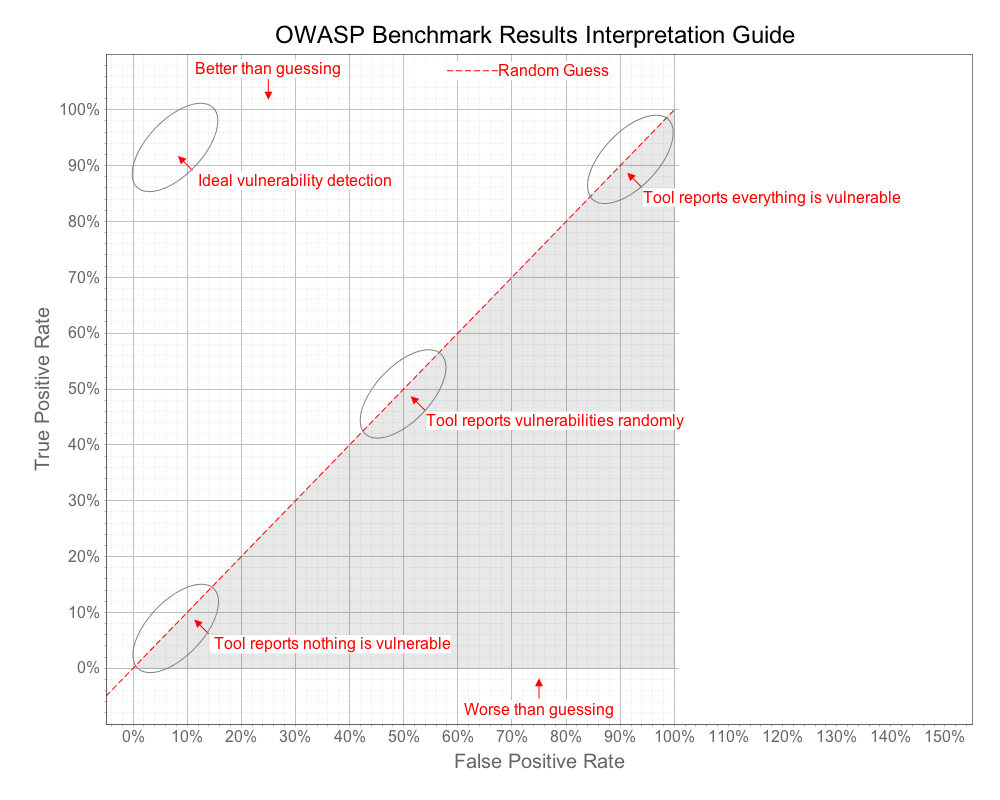
\includegraphics[width=.7\linewidth]{images/benchmark_guide.png}
%     \caption{OWASP Benchmark Scoring Guide - Youden Index interpretation \cite{owasp_benchmark_scoring}}
%     \label{fig:owasp_benchmark_scoring}
% \end{figure}

%%%% PERFORMANCE

By running KLEE and Owi on the same set of samples, some differences are visible in their outputs and in their performances (see \Cref{tab:klee_performance,tab:owi_performance}). KLEE was overall slower, with the only exception being the primes example, but was also the example that consumed less CPU but also Memory on all samples.

Unfortunately, Owi does not seem to output information regarding the travelled states, even after looking at debug logs (which depict execution instructions, but nothing was found to support a number of traversed paths).

An example of how the performance between these tools differ is with sample 3, a test where KLEE traces 306 paths. KLEE reported results consuming nearly half the CPU resources and approximately 73\% of the memory usage and 35\% of the time spent, that Owi required to run and return no results on the sample.

Sample 2 shows an even greater difference; KLEE spends nearly half the CPU and 19\% of the memory usage when compared to Owi, and does that in 1\% of the time it took Owi to analyse the same source. This scenario might be a clear indicator of Owi limitations.

% \newpage
% KLEE tests table
\begin{table}[tb]
    \begin{center}
    \caption{KLEE performance metrics}
    \begin{tabular}{c|c|c|c|c|c}
        \#$^{\mathrm{a}}$ & Success & Paths traced & CPU \textsubscript{(\%)} & Memory \textsubscript{(KB)} & Time \textsubscript{(s)}$^{\mathrm{b}}$ \\
        \hline
        \hline
        1 & YES & 3 & 99 & 98'156 & 0.29 \\
        2 & YES & 6'675 & 101 & 139'680 & 12.93 \\
        3 & YES & 305 & 93 & 99'152 & 0.72 \\
        4 & YES & 99 & 98 & 99'504 & 2.93 \\
        5 & YES & 1 & 81 & 98'036 & 0.39 \\
        6 & YES & 5 & 102 & 98'920 & 0.30 \\
        7 & YES & 5 & 87 & 97'536 & 0.37 \\
        8 & YES & 5 & 96 & 98'248 & 0.33 \\
        9 & YES & 5 & 96 & 99'236 & 0.32 \\
        \hline
        \multicolumn{6}{l}{}\\
        \multicolumn{6}{l}{$^{\mathrm{a}}$\footnotesize{Sample number}} \\
        \multicolumn{6}{l}{$^{\mathrm{b}}$\footnotesize{The best out of five runs}}
    \end{tabular}
    \end{center}
    \label{tab:klee_performance}
\end{table}

% Owi tests table
\begin{table}[tb]
    \begin{center}
    \caption{Owi performance metrics}
    \begin{tabular}{c|c|c|c|c|c}
        \#$^{\mathrm{a}}$ & Success & Paths traced & CPU \textsubscript{(\%)} & Memory \textsubscript{(KB)} & Time \textsubscript{(s)}$^{\mathrm{b}}$ \\
        \hline
        \hline
        1 & YES & \textcolor{gray}{N/A} & 108 & 110'000 & 0.05 \\
        2 & YES & \textcolor{gray}{N/A} & 200 & 725'892 & 901.51 \\
        3 & YES & \textcolor{gray}{N/A} & 199 & 134'928 & 2.10 \\
        4 & YES & \textcolor{gray}{N/A} & 204 & 145'676 & 9.90 \\
        5 & YES & \textcolor{gray}{N/A} & 205 & 151'800 & 11.13 \\
        6 & YES & \textcolor{gray}{N/A} & 116 & 120'172 & 0.06 \\
        7 & YES & \textcolor{gray}{N/A} & 115 & 119'172 & 0.06 \\
        8 & YES & \textcolor{gray}{N/A} & 118 & 118'220 & 0.05 \\
        9 & YES & \textcolor{gray}{N/A} & 123 & 121'040 & 0.05 \\
        \hline
        \multicolumn{6}{l}{}\\
        \multicolumn{6}{l}{$^{\mathrm{a}}$\footnotesize{Sample number}} \\
        \multicolumn{6}{l}{$^{\mathrm{b}}$\footnotesize{The best out of five runs}}
    \end{tabular}
    \end{center}
    \label{tab:owi_performance}
\end{table}


\section{CONCLUSION}\label{chap:conclusion}

The performed testing allowed us to establish how each tool compares in terms of speed, and CPU and memory usage. Not only that, but a quick glance of what each tool offers clearly demonstrates how Owi was designed as an extremely helpful toolkit for \acrshort{wasm} development, with all of the subcommands bundled, that enables developers to integrate symbolic execution into their \gls{sdlc} cycle.% and therefore increase their test coverage.

KLEE, on the other hand, is purely designed to be a symbolic execution engine that proved itself by making use of a symbolic environment and developing a good solution on path explosion can improve the tool's efficiency.

To take this research and method a step further a couple of improvements could be taken such as: testing in a dedicated test machine instead of the available alternative (laptop); increasing sample size both in number as in individually larger code samples, examples to this are the Test-Comp benchmarks; and lastly, increasing the number of tested symbolic execution tools.

In conclusion, this work aims at making symbolic execution a familiar concept in the life of a software developer; despite the investigated tools being oriented to specific development platforms, the examined samples were not, proving we can still compile programs to an architecture that is not the intended for a `production environment' and have good testing mechanisms.

\subsection{Research Questions}

The defined \nameref{section:objectives} (\cref{section:objectives}) for this work were mostly answered in \cref{section:results} \nameref{section:results} with \Crefrange{tab:klee_accuracy}{tab:owi_performance} and \cref{equ:klee_youden_index,equ:owi_youden_index}. All performance questions are answered in \Cref{tab:klee_performance,tab:owi_performance} and the tools accuracy metrics are also tracked and calculated in \Cref{tab:klee_accuracy,tab:owi_accuracy}, and \cref{equ:klee_youden_index,equ:owi_youden_index}. Each topic was answered for both KLEE and Owi.

The metrics collected helped conclude that KLEE was overall superior both in performance and in its bug-finding capabilities. Despite being superior at finding vulnerabilities, KLEE still scores poorly in the OWASP Benchmark scoring table (54\%) \cite{owasp_benchmark_scoring}, mainly due to its False Positive Rate, but the real culprit of this result is the size of the test sample.

There are still, however, some unanswered questions:
\begin{itemize}
	\item \textbf{Complexity of the vulnerabilities detected}\\
	To properly answer this question additional work is required; the samples analysed in \cref{chap:experiences} are of low complexity and therefore there isn't much room for complexity of vulnerabilities.
	\item \textbf{Ability to find vulnerabilities out-of-the-box}\\
	Neither tool seemed to be able to find bugs without tampering with the program sources, but that is mainly because of the very nature of symbolic execution and how the engine must know which variables are symbolic so it can travel execution paths and attempt to discover runtime problems.
	However, if we only consider tool configurations, no extra argument or special execution of KLEE or Owi is required to find problems (once the sources are properly instrumented).
	\item \textbf{Ability to find vulnerabilities with proper manipulation}\\
	Similarly to the previous question, because of the very nature of symbolic execution, we're required to edit source files so the engines are able to do their jobs.
	In terms of custom arguments for the tools, some arguments like KLEE's \lstinline$--uclibc$ and Owi's \lstinline$-w$ might help in achieving results by either providing additional context or providing concurrent scanning.
	\item \textbf{Effort of tuning the tool}\\
	Both utilities require source modifications but without major complexities, but KLEE functions are more ergonomical than Owi's.
\end{itemize}

In \cref{section:research_method} \nameref{section:research_method} some questions regarding performance and accuracy are expanded. Others are reiterated to reinforce lessons learned:

\begin{itemize}
	\item \textbf{Is the tool useless without proper tuning?} \\
	Both KLEE and Owi require information on the scanned sources, without any information the testing will be very limited. However, this is not a limitation of the tools but of the analysis method.
	\item \textbf{How does the Youden's Index compare?} \\
	\Cref{equ:klee_youden_index,equ:owi_youden_index} show better results in favour of KLEE despite the small size of the test sample. According to \citeauthor{owasp_benchmark_scoring} \cite{owasp_benchmark_scoring}, KLEE's score of 54\% is considered as good as random guessing and Owi's 29\% mean nearly nothing is considered vulnerable code. Again, these results are a reflection of the small size of the test cases.
\end{itemize}

All these answers help answering the main research questions defined in \cref{section:objectives} \nameref{section:objectives}.
KLEE is overall most effective at finding vulnerabilities and also the more efficient in terms of performance.

\section{ACKNOWLEDGMENTS}

XXX

% \section*{References}

\bibliographystyle{IEEEtranN}
\bibliography{IEEEabrv,library}

\end{document}
